\chapter{Discretization}\label{chapter:discretization}
Having discussed the NSE and the different kinds of rearrangements and simplifications, we completed the first two steps of \emph{modeling} and \emph{approximating}.
Next, we address the problem of simulating the NSE on computers with finite memory and computational capacity.
To this end, we must discretize all the continuous spatial and temporal terms in the NSE, in order to make the memory and time required for computation finite.
These discretizations account for Step 3 (\emph{Space Discretization}) and Step 4 (\emph{Time Discretization}) of solving a PDE numerically.

The meaning of discretization can be seen by looking at one of the equations to be discretized:
\begin{align*}
\frac{\partial w}{\partial t} &= -g\left(1 - \frac{\partial p}{\partial s}\left(\frac{\partial \pi}{\partial s}\right)^{-1}\right)
\end{align*}
First, spatial derivatives and other spatial differential operators like $\frac{\partial p}{\partial s}$ must be discretized, i.e. they must be approximated.
This must be done using a finite number of samples of $p$ around the point where the derivative is to be calculated.

Second, $w$ and $p$ must be discretized themselves.
In the real world these are continuous in space.
However, when computing, we can only represent them with a finite number of samples.
Usually, every variable in a differential equation is assigned to a grid, and at every node of that grid a measurement of the variable is stored.

Third, we must discretize the time variable in $\frac{\partial w}{\partial t}$.
To be more specific, we need to reverse the time derivative, i.e. integrate it, in order to gain the real value of $w$ from the diagnostic equation for $\frac{\partial w}{\partial t}$.

In summary, we assume the state of the system at time $t$ to be represented by a number of variables stored in the nodes of a grid.
Next we evaluate the value of the differential equation at those grid nodes.
We approximate any spatial derivative required for this through its respective discrete spatial derivative.
For these discrete spacial derivatives we only make use of the variable values at the grid points.
To approximate the state of the system at some other discrete time $t+\Delta t$, we then input the value of the differential equation to an integrator which reverses the time derivative.

\subsubsection{Overview}
In Section~\ref{section:diff_op} we address the discretization of differential operators.
In Section~\ref{sec:grid_discretization} we discuss the important issue of discretization of prognostic variables onto a regular grid.
In Section~\ref{sec:integrators} we present the integration operators which we implemented for this thesis.

\section{Discretization of Differential Operators}\label{section:diff_op}
In this section we present two methods for approximating spatial derivatives using only samples at discrete spatial locations.
The first method is called finite differences and approximates the derivative at a location by only looking at samples close to that location.
While not always the most accurate, this method makes no assumptions\footnote{except for sufficient differentiability} about the function it is taking the derivative of.

The second method (sometimes called spectral) takes a detour to the frequency domain to approximate the derivative.
While this method is highly accurate when applicable, it assumes the boundary conditions to be periodic.
This is not the case for the vertical dimension of weather simulation, hence we cannot employ this method for simulating the vertical dimension of the NSE.
We present it nonetheless, because it plays a central role for numerical weather prediction in the horizontal dimension.

\subsection{Finite Differences}
In order to derive the commonly known (e.g. refer to~\cite{smith1985numerical}) finite difference operators, we must introduce the Taylor Series.
It approximates a function around a given point with polynomials and spatial derivatives as follows.

Let $f:\mathbb{R}\times\mathbb{R}^q\rightarrow \mathbb{R}$ be a function which we want to develop along its first argument $x$.
All other inputs $\boldsymbol{v}$ are held constant.
Employing the Landau notation, and with $\mathcal{O}(\Delta x ^{n+1})$ being the error of the approximation, the following holds:
\begin{equation}
f(x+\Delta x,v) = \sum_{k=0}^{n}\frac{1}{k!}\cdot\frac{\partial^k f}{\partial x ^k}(x,v)\cdot \Delta x^k + \mathcal{O}(\Delta x ^{n+1})
\end{equation}
Assuming an equidistant grid, i.e. the values of $f(x+k\Delta x,v)$ for $k\in [-l,u] \cap \mathbb{Z}$ are known, this yields a linear equation system of size $l + u + 1 - 1= l + u$ ($-1$ because $k=0$ yields no information).
In the following, we omit the second argument $v$ in the equations.

\begin{align*}
f(x - l \Delta x) &= f(x) + \frac{1}{1!}\cdot\frac{\partial f}{\partial x}(x)\cdot (-l\Delta x)^1 + \frac{1}{2!}\cdot\frac{\partial^2 f}{\partial x^2}(x)\cdot (-l\Delta x)^2 + ... + \mathcal{O}((\Delta x) ^{l+u+1})\\
&...\\
f(x) &= f(x) + \frac{1}{1!}\cdot\frac{\partial f}{\partial x}(x)\cdot (0)^1 + \frac{1}{2!}\cdot\frac{\partial^2 f}{\partial x^2}(x)\cdot (0)^2 + ... + \mathcal{O}((0) ^{l+u+1})= f(x)\\
&...\\
f(x + u \Delta x) &= f(x) + \frac{1}{1!}\cdot\frac{\partial f}{\partial x}(x)\cdot (u\Delta x)^1 + \frac{1}{2!}\cdot\frac{\partial^2 f}{\partial x^2}(x)\cdot (u\Delta x)^2 + ... + \mathcal{O}((\Delta x) ^{l+u+1})\\
\end{align*}
The equation system consists of $l+u$ unknowns, i.e. $\frac{\partial^k f}{\partial x^k}(x,v)$, and $l+u$ equations.
The error of the approximation made by solving for one of the unknowns $\frac{\partial^k f}{\partial x^k}(x,v)$ is $\mathcal{O}((\Delta x) ^{l+u+1-k})$ ($-k$ comes from the fact that the equation must be divided by $\Delta x ^k$ before being solved).
In this thesis we mostly apply the first derivative.
To this end, we mostly use the following four configurations which are also visualized in Fig.~\ref{fig:finite_differences}:

\begin{figure}[!h]
	\makebox[\textwidth]{ 
  		 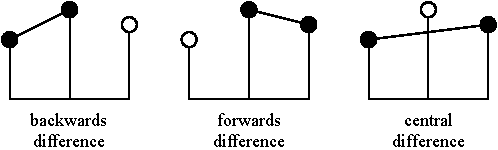
\includegraphics[width=0.9\textwidth]{figures/forwards_backwards_central.pdf}}
    \caption{Visualization of forwards ($l=0,u=1$), backwards ($l=1,u=0$), and central differences ($l=1,u=1$)}
    \label{fig:finite_differences}
\end{figure}

\begin{align*}
l=0,u=1&: \frac{\partial f}{\partial x}(x) = \frac{f(x+\Delta x) - f(x)}{\Delta x} + \mathcal{O}((\Delta x)^{1})\\
l=1,u=0&: \frac{\partial f}{\partial x}(x) = \frac{f(x) - f(x-\Delta x)}{\Delta x} + \mathcal{O}((\Delta x)^{1})\\
l=1,u=1&: \frac{\partial f}{\partial x}(x) = \frac{f(x + \Delta x) - f(x-\Delta x)}{2\Delta x} + \mathcal{O}((\Delta x)^{2})\\
l=2,u=2&: \frac{\partial f}{\partial x}(x) = \frac{f(x-2\Delta x) -8 f(x-\Delta x) + 8 f(x+\Delta x) - f(x+2\Delta x)}{12\Delta x} + \mathcal{O}((\Delta x)^{4})\\
\end{align*}


\subsection{Spectral Methods for Periodic Boundary Conditions}
While finite differences are quite intuitive in their nature, the derivative of a function can also be calculated by spectral methods.
For the method presented here, this requires periodic boundary conditions and entails the usage of the Fourier Transform.
According to Johnson~\cite{johnson2011notes}, the intuition behind this can be seen by assuming that any function on a domain $[0;L]$ can be written as a series:
\begin{align*}
y(x) = \sum_{k=-\infty}^{\infty}Y_k\exp \left(\frac{2\pi i}{L}kx\right)
\end{align*}
Given that all $Y_k$ are known, the derivative $\frac{dy}{dx}$ can be written as a new series:
\begin{align*}
\frac{dy}{dx}(x) = \sum_{k=-\infty}^{\infty}\left(\frac{2\pi i}{L}kY_k\right)\exp \left(\frac{2\pi i}{L}kx\right)
\end{align*}
In this example the coefficients $Y_k$ are the Fourier Transform of $y(x)$, and the coefficients $(\frac{2\pi i}{L}kY_k)$ are the Fourier Transform of the derivative $\frac{dy}{dx}(x)$.
As there is clearly a linear relationship between the Fourier coefficients of the function and the coefficients of its derivative, the derivative of any function can be calculated in three steps:
First, calculating the Fourier coefficients of a function.
Second, modifying the calculated Fourier coefficients appropriately.
Third, calculating the derivative by applying the inverse Fourier Transform on the the modified Fourier coefficients, i.e. by calculating $\frac{dy}{dx}(x)$ from $(\frac{2\pi i}{L}kY_k)$.

Given the fact that computers are not dealing with continuous functions, but only with discrete samples thereof, we must apply the discrete Fourier Transform.
It is commonly calculated by means of the Fast Fourier Transform (FFT).
The derivation of this method can be found in~\cite{johnson2011notes}.
\\

The main advantage of this spectral method is its precision as long as the spatial sampling rate is sufficiently high\footnote{In signal-processing terms the sample frequency must exceed the Nyquist frequency, and in this case the accuracy is only limited by numerical effects, such as machine precision}, as will be seen in the numerical testing done in Section~\ref{sec:numeric_diff_ops}.

However, the downsides to this method are twofold.
First, the method requires boundary conditions to be periodic in order to work, because the FFT assumes periodic boundary conditions.
Second, computing the FFT takes $\mathcal{O}(n\log n)$ which is significantly slower than the $\mathcal{O}(n)$ required for finite difference operators.

We introduced the spectral methods nontheless, because they are common when simulating the horizontal dimension of the weather system on a planetary scale~\cite{coiffier2011fundamentals},\cite{chen1997use},\cite{shuman1989history}.
This is possible because in the horizontal dimension a spherical planet has periodic boundary conditions.
That is, if one were to always travel exactly eastward endlessly, one would end up where one started periodically.
In other words, the endless journey eastward is periodic and so are the boundary conditions of the horizontal system.

\section{Grid Discretizations}\label{sec:grid_discretization}
\begin{figure}[ht]
	\makebox[\textwidth]{ 
  		 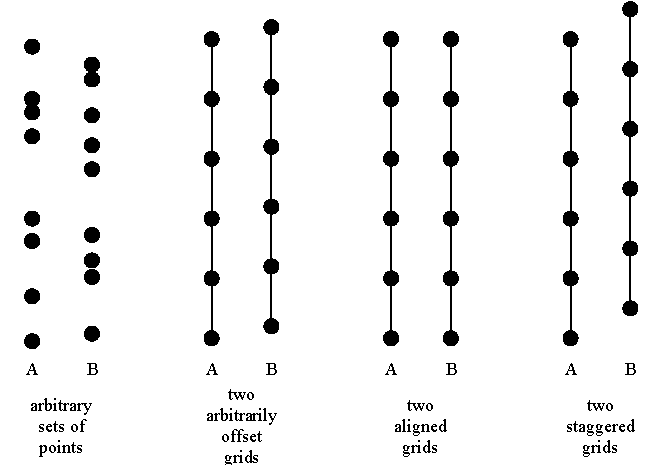
\includegraphics[width=.8\textwidth]{figures/discretization.pdf}}
    \caption{Different variants of discretization}
    \label{fig:grid_discretization}
\end{figure}
\begin{figure}[ht]
	\makebox[\textwidth]{ 
  		 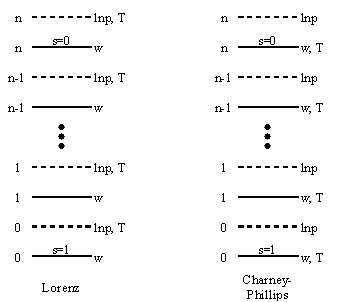
\includegraphics[width=.7\textwidth]{figures/lorenz_cp.pdf}}
    \caption{Variable distribution for Lorenz grid and Charney-Phillips grid}
    \label{fig:lorenz_cp}
\end{figure}
\noindent
When implementing the non-hydrostatic version of the NSE discussed in Section~\ref{sec:non_hydrostatic}, there are three prognostic variables to be considered: Vertical wind speed $w$, pressure $\text{ln}p$, and temperature $T$.
Each of them varies across the atmosphere and must thus be sampled at different points across space.
The question is where to place these points for each variable.

Generally speaking, every variable gets its own arbitrary set of points at which to sample.
In theory, the set of points could also vary over time.

To simplify calculation, we apply grids to bring order to the sets of points.
When a variable is sampled along a grid, it is sampled at every node of that grid.
In order to utilize the discrete differential operators from Section~\ref{section:diff_op}, the grids are chosen to be equidistant, i.e. the distance between two consecutive grid points (the mesh size) is always the same.
It is also assumed that the mesh size is the same for all three variables.

Note that in this context, the distance between grid points does not necessarily correspond to distance (measured in meters) in the real world.
This is due to the alternative coordinate system from Section~\ref{sec:non_hydrostatic} which transforms equidistant grid points in the s-coordinate-system to non-equidistant grid points in the z-coordinate system, depending on how the function $\pi(s)$ is defined.
This effect can be observed in Fig.~\ref{fig:s_grid}.
\begin{figure}[ht]
	\makebox[\textwidth]{ 
  		 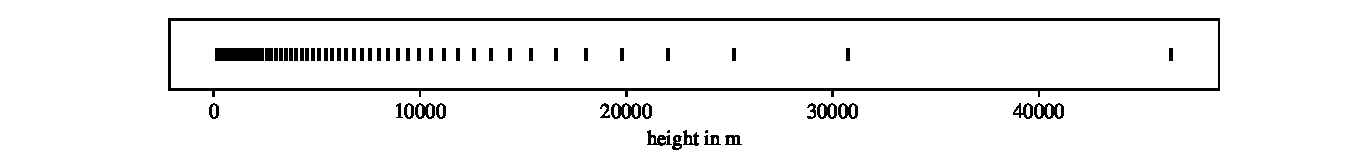
\includegraphics[width=.9\textwidth]{figures/50gridpoints.pdf}}
  	\makebox[\textwidth]{ 
  		 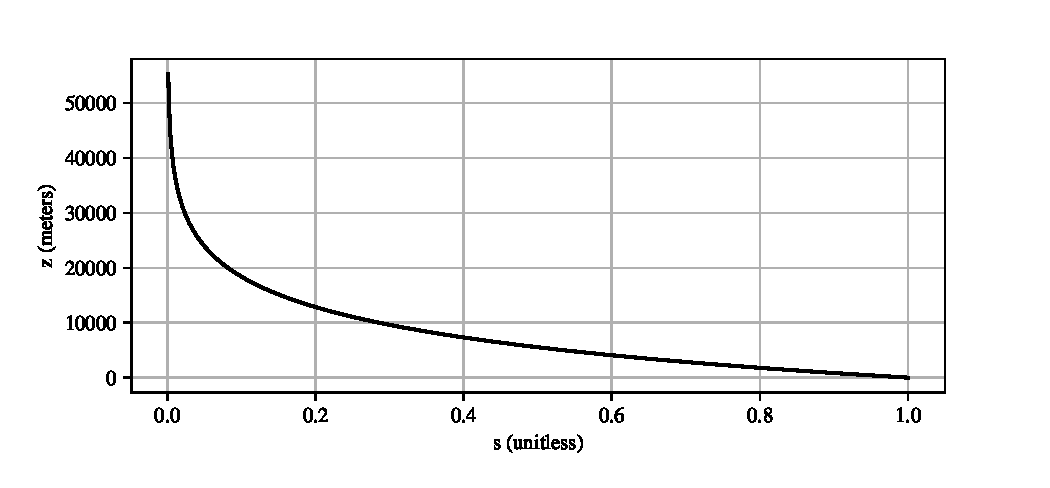
\includegraphics[width=.9\textwidth]{figures/s_to_z.pdf}}
    \caption{Transformation of $s$-coordinates to $z$-coordinates;
    both diagrams assume that $\pi (s)=s\cdot 1atm$, and $T=273K$, and use Eq.~\ref{eq_s_to_z} to translate an equidistant $s$-grid to a non-equidistant $z$-grid.
    The first diagram shows where each grid point is located in $z$-coordinates with $50$ grid points. 
    The second diagram shows the relationship between $s$-coordinates and $z$-coordinates.}
    \label{fig:s_grid}
\end{figure}

Having now established that all three variables ($\text{ln}p$, $T$, and $w$) are sampled along grids of equal mesh size, one remaining question is their relative placement.
In other words, the offset between two grids for two variables is a free parameter.
In case the offset is zero, we call the two grids aligned.
In case the offset is half the distance between two grid points, the two grids are called staggered.
To distinguish the two grids, we call one aligned, and the other offset.
This is illustrated in Fig.~\ref{fig:grid_discretization}.

For the NSE there are two prevailing staggered grid systems~\cite{holdaway2013comparison}: The Lorenz grid, and the Charney-Phillips grid which are shown in Fig.~\ref{fig:lorenz_cp}.
For the Lorenz grid, vertical wind $w$ is placed on the aligned grid, whereas pressure $\text{ln}p$ and temperature $T$ are on the offset grid.

For the Charney-Phillips grid, both vertical wind $w$ and temperature $T$ are placed on the aligned grid, and only pressure $\text{ln}p$ is on the offset grid.
The reason for always placing $w$ on the aligned grid, and pressure $\text{ln}p$ on the offset grid, is to enforce the boundary conditions discussed in Section~\ref{sec:boundary}.
By placing wind $w$ on the aligned grid, we can force $w_{top}$ and $w_{bottom}$ to be zero, since there are sample points both at the top and the bottom.

In contrast, with pressure $\text{ln}p$ it is advantageous not to have a sampling point at the upper boundary of the domain, as we may want to postulate pressure at the upper boundary to be zero, because the atmosphere is supposed to end there, i.e. $p_{top}=0$ which would mean $\text{ln}p = -\infty$.
To avoid dealing with non-computable numbers, pressure $\text{ln}p$ is placed on the offset grid.

We can place the remaining variable temperature $T$ on either the offset or the aligned grid, because it not affected by our boundary conditions.

\section{Discretization of Time and Types of Integrators}\label{sec:integrators}
Before we give examples of integrators, we must first define them.
An integrator is an algorithm that, given a starting condition $x(t_0) = x_0$, can solve a differential equation of the form $\frac{dx}{dt} = f(x,t)$, where $x$ is the state vector and $t$ is time.
Its goal is to generate a trace for $x(t)$ over time, after the starting time $t_0<t$.

\subsection*{Runge-Kutta Methods}
One of the simpler classes of integrators consists of the explicit Runge-Kutta methods.
These methods begin with the initial value $x_0$ and then create the trace $x(t)$ by making small time-steps $\Delta t$ starting at $t_0$ and modifying the state through addition: $x(t+h) = x(t) + RK(f,x,t,h)$.

The following derivation closely follows the derivation in~\cite{lyu2016plasma}.
Other derivations such as in~\cite{suli2003introduction} are also possible.
\\

\noindent
All Runge-Kutta methods aim to approximate the Taylor series expansion of $x(t)$ with respect to $t$, i.e.
\begin{align*}
x(t+h) &= x(t) + \sum_{k=1}^{n}\frac{h^k}{k!}\frac{d^kx}{dt^k} + \mathcal{O} \left(h^{n+1}\frac{d^{n+1}x}{dt^{n+1}}\right)\\
&= x(t)+ \sum_{k=0}^{n-1}\frac{h^{k+1}}{(k+1)!}\frac{d^kf(x(t),t)}{dt^k} + \mathcal{O}\left(h^{n+1}\frac{d^{n}f}{dt^{n}}\right)
\end{align*}
Exploiting $\frac{df(x(t),t)}{dt} 
= \frac{\partial f(x(t),t)}{\partial x}\frac{dx}{dt}+\frac{\partial f(x(t),t)}{\partial t} 
= f\frac{\partial f}{\partial x}+\frac{\partial f}{\partial t}$
this becomes.
\begin{align*}
x(t+h) &= x(t)+ \sum_{k=0}^{n-1}\frac{h^{k+1}}{(k+1)!}\left(\frac{\partial f}{\partial t} + f(x(t),t)\frac{\partial f}{\partial x}\right)^kf(x(t),t) + \mathcal{O}\left(h^{n+1}\frac{d^{n}f}{dt^{n}}\right)
\end{align*}
The simplest Runge Kutta method is the Explicit Euler or RK1 scheme which can be derived by writing down the Taylor expansion:
\begin{align*}
x(t+h) &= x(t) + h \cdot \frac{dx}{dt} + \mathcal{O}(h ^2)\\
&= x(t) + h \cdot f(x,t) + \mathcal{O}(h ^2)
\end{align*}
RK1 has a local truncation error of $\mathcal{O}(h^2)$, and a total accumulated error of $\mathcal{O}(h)$.
\\

\noindent
RK2 uses more than one evaluation of $f$ in order to do one step:
\begin{align*}
k_1 &= f(x(t),t)\\
k_2 &= f(x(t) + \frac{h}{2} k_1, t + \frac{h}{2})\\
&= f(x(t) + \frac{h}{2} f(x(t),t), t + \frac{h}{2})\\
&= f(x(t),t) + h\left(\frac{\partial f}{\partial t} + f(x(t),t)\frac{\partial f}{\partial x}\right)f(x(t),t) + \mathcal{O}(h^2)\\
&= f(x(t),t) + h\frac{df}{dt} + \mathcal{O}(h^2)\\
x(t) + \frac{h}{2} (k_1+k_2) &= x(t) + \frac{h}{2} \left(f(x(t),t) + f(x(t),t) + h\frac{df}{dt} + \mathcal{O}(h^2)\right)\\
&= x(t) + h f(x(t),t) + \frac{h^2}{2} \frac{df}{dt} + \mathcal{O}(h^3)\\
&= x(t) + h \frac{dx}{dt} + \frac{h^2}{2} \frac{d^2x}{dt^2} + \mathcal{O}(h^3)\\
\Rightarrow x(t+h) &= x(t) + \frac{h}{2} (k_1+k_2) + \mathcal{O}(h^3)
\end{align*}
RK2 has a local truncation error of $\mathcal{O}(h^3)$, and a total accumulated error of $\mathcal{O}(h^2)$.
\\

\noindent
In a similar fashion it can be shown that RK4 is:
\begin{align*}
k_1 &= f(x(t),t)\\
k_2 &= f\left(x(t)+\frac{h}{2}k_1,t+\frac{h}{2}\right)\\
k_3 &= f\left(x(t)+\frac{h}{2}k_2,t+\frac{h}{2}\right)\\
k_4 &= f(x(t) + h k_3, t + h)\\
x(t+h) &= x(t) + \frac{h}{6}(k_1+2k_2+2k_3+k_4)
\end{align*}
RK4 has a local truncation error of $\mathcal{O}(h^5)$, and a total accumulated error of $\mathcal{O}(h^4)$.

%\subsection{Exponential Integrators}
%In case $f(x,t)$ is a linear timeinvariant function, $f$ can be written as $f(x)=Ax$, where $A$ is a matrix.
%The resulting differential equation can be solved analytically, using the Laplace Transform which is explained in further detail in appendix \ref{sec:laplace_trafo}.
%To this end first, the Laplace transform is taken, and then the equation is solved for $X(s)$ (with $I$ being the identity matrix):
%\begin{align*}
%\frac{dx}{dt}(t) &= Ax(t)\\ 
%sX(s) - x(t_0) &= AX(s)\\
%X(s) &= (sI-A)^{-1}x(t_0)
%\end{align*}
%Thereafter the inverse Laplace transform can be taken to solve for $x(t)$:
%\begin{align*}
%x(t) &= \exp (A (t-t_0))x(t_0)\\
%\text{using:}~ \exp{At} &= I + \sum_{k=1}^{\infty}\frac{1}{k!}(At)^k
%\end{align*}
%As this is an analytic solution, it is exact and does not depend on step-size.
%However there are two major disadvantages to this method.
%First, if the system is not linear it needs to be linearized which makes the solution inexact.
%Second, it is comparatively slow as it requires a matrix to be exponentiated.
%Take, for example, the NSE discussed earlier.
%If temperature, wind speed, and density are stored at just 3000 grid points, this would entail the state vector $x$ having at least $3000\cdot 3=9000$ entries, and thus $A$ having $9000^2=8.1\cdot 10^7$ entries which would still be feasible to compute, just not fast, especially when compared to Runge-Kutta methods.\\
%As a countermeasure to the second issue, the matrix exponential can be approximated using several approaches.
%For further reading on this topic refer to~\cite{moler2003nineteen}.

%\begin{itemize}
%\item show how linear equations can be solved using laplace-%transforms and matrix exponentials
%\item give example of how matrix exponential can be approximated
%\end{itemize}

